\documentclass[10pt, a4paper]{beamer}
\usepackage{subcaption}
\usepackage{graphicx}
\usepackage{listings}
\usetheme{Berkeley}
\usecolortheme{sidebartab}

\begin{document}
	\setbeamertemplate{sidebar left}{}
	\title{Progress Presentation-I}
	\subtitle{e-Yantra Summer Intership-2016 \\ Raspberry Pi Hardware Development and Tutorials}
	\author{Aditya Kumar\\Pritish P Salunke\\
	Mentor: Rutuja E \\ Deepa A}
	\institute{IIT Bombay}
	\date{\today}
	%\addtobeamertemplate{sidebar left}{}{\includegraphics[scale = 0.3]{logowithtext.png}}
	\frame{\titlepage}

\setbeamertemplate{sidebar left}[sidebar theme]
\section{Overview of Project}
\begin{frame}{Overview of Project}
	\begin{itemize}
		\item Project Name: Raspberry Pi Hardware Development and Tutorials
		\item Objective
		\begin{enumerate}
			\item Test available modules of Raspberry Pi
			\item Generate new modules
			\item Communication between Firebird V and RPi
			\item Design stackable PCB for each module
		\end{enumerate}
		\item Deliverables
		\begin{enumerate}
			\item Hardware along with circuit schematics and PCB
			\item Code and Documentation to interface each components
			\item Video tutorials explaining individual module
		\end{enumerate}
	\end{itemize}
\end{frame}

\section{Overview of Task}
\begin{frame}{Overview of Task}
		\begin{center}
			\begin{tabular}{|c|c|c|}
				\hline
				Task No. & Task & Deadline\\
				\hline
				1 & Learn available Modules on RPi. &  4 days \\ & Create video tutorials. &     \\ 
				\hline
				2 & Zigbee and Bluetooth Communication. & 5 days\\ & Create video tutorials and documentation &  \\
				\hline
				3 & Communication between RPi and Firebird V & 4 Days \\ & using I2C, UART and SPI. &\\ & Create video tutorials and Documentation  & \\
				\hline
				4 & Interface LCD.& 3 Days\\ & Create video tutorials and documentation. & \\
				\hline
				5 & Mapping of all Firebird V & 5 Days\\ & example programs in Python & \\
				\hline
				6 & PCB Design & 5 Days \\
				\hline
				7 & Challenge Activity & 3 Days\\
				\hline
			\end{tabular}
		\end{center}
\end{frame}

\section{Task Accomplised}
\begin{frame}{Task Accomplised}
	\begin{itemize}
		\item Accessing GPIO pins on RPi
		\item Interfacing port expander
		\item Communication between Rpi and devices using I2C,
		      SPI protocol
		\item ADC interfacing \\Temp. Sensor, Sharp sensor MCP3008
		\begin{figure}[h!]
			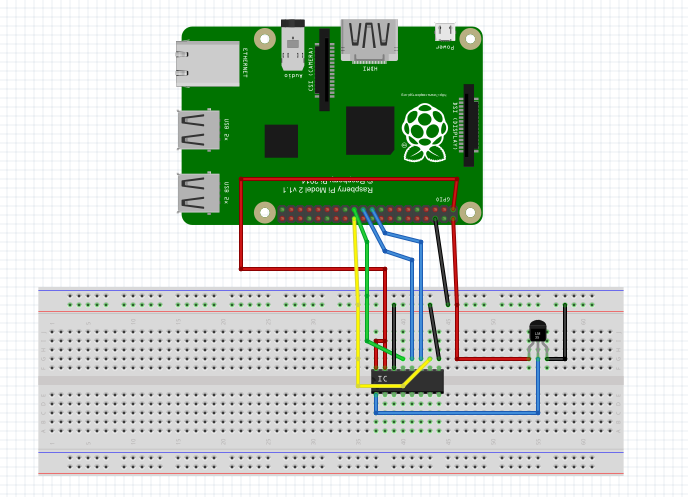
\includegraphics[scale=0.3]{lm35_interfacing.jpg}
			\centering
			\caption{Connection for interfacing LM35}
		\end{figure} 
	
	\end{itemize}
\end{frame}
\begin{frame}{Task Accomplished}
	\begin{itemize}
		\item Interfacing dc and sevo motor
		 \begin{figure}[h!]
		 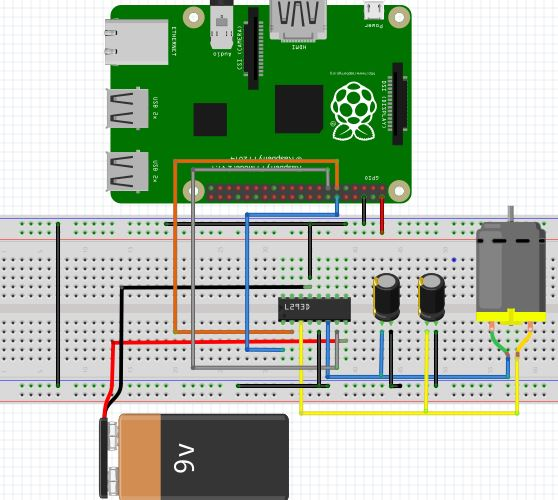
\includegraphics[scale=0.3]{DC_motor_GPIO.jpg}
		 \centering
		 \caption{Connection on breadboard for dc motor}
		\end{figure}
	\end{itemize}
\end{frame}
\begin{frame}{Task Accomplished}
	\begin{itemize}
		\item Zigbee and Bluetooth Communication
		\begin{figure}[h!]
			\begin{subfigure}{0.5\textwidth}
				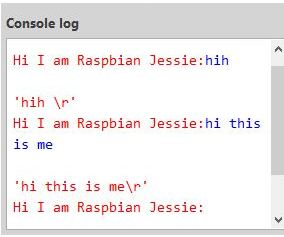
\includegraphics[width=0.7\linewidth,height=2.5cm]{Xctu1.jpg}
				\centering 
				\caption{Output on XCTU}
			\end{subfigure}
			\begin{subfigure}{0.5\textwidth}
				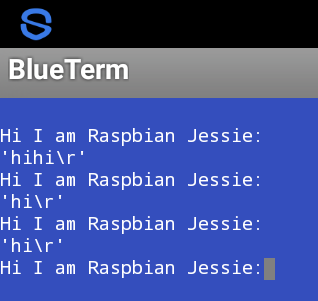
\includegraphics[width=0.6\linewidth,height=2.5cm]{Blueterm1.jpg}
				\centering
				\caption{Output on Blueterm}
			\end{subfigure}
		\end{figure}
	\end{itemize}
\end{frame}

\section{Challenges Faced}
\begin{frame}{Challenges Faced}
	\begin{itemize}
		\item List challenges faced while accomplishing the task.  
	\end{itemize}
\end{frame}

\section{Future Plans}
\begin{frame}{Future Plans}
	\begin{itemize}
		\item List deliverables for next progress presentation  
		\item PCB sheilds for each module
		\item Documentation for communication between Rpi and FireBird V
		\item Example programs in python
		\item Video Tutorial for all the tasks 
	\end{itemize}
\end{frame}


\section{Thank You}
\begin{frame}{Thank You}
	\centering THANK YOU !!!
\end{frame}
\end{document}
